
%(BEGIN_QUESTION)
% Copyright 2009, Tony R. Kuphaldt, released under the Creative Commons Attribution License (v 1.0)
% This means you may do almost anything with this work of mine, so long as you give me proper credit

Calculate the percentage of incident power reflected back to the transmitter, and the percentage of incident power transmitted (forward) through the liquid in this radar level measurement application:

$$\includegraphics[width=15.5cm]{i00034x01.eps}$$

Also, calculate the ullage for this vessel in units of feet, given a reflected pulse (``echo'') time of 17.0 nanoseconds.  Assume a speed of light in vacuum to be $3 \times 10^8$ meters per second.  For all your answers, be sure to show your work!

\vskip 30pt

$P_{reflected}$ = \underbar{\hskip 50pt} \%

\vskip 70pt

$P_{forward}$ = \underbar{\hskip 50pt} \%

\vskip 70pt

Ullage = \underbar{\hskip 50pt} ft

\underbar{file i00034}
%(END_QUESTION)





%(BEGIN_ANSWER)

$P_{reflected}$ = \underbar{\bf 20.38} \%

\vskip 10pt

$P_{forward}$ = \underbar{\bf 79.62} \%

\vskip 10pt

Ullage = \underbar{\bf 8.366} ft

%(END_ANSWER)





%(BEGIN_NOTES)


%INDEX% Measurement, level: radar

%(END_NOTES)


